
\section{Experiments}\label{sec:experiments}

\subsection{Protocol}\label{sec:protocol}

Every experiment streams data in batches and inspects the estimate after every
batch, scoring the \emph{worst case over the whole trajectory} rather than the
state at a single sample size. This is deliberate: a time-uniform guarantee is
a claim about trajectories, and evaluating it at a single $n$ would measure
something else. Where a comparator has only a fixed-sample guarantee we report
both its trajectory-worst behaviour (which is what an analyst monitoring it
would experience) and its behaviour at the final sample size (which is what
its guarantee covers), because reporting only the first would be unfair and
reporting only the second would miss the point.

Random DAGs are drawn with independent edge probabilities in a random
topological order, with coefficients uniform on $\pm[0.5, 1.2]$. Noise is
Laplace unless stated. Binomial proportions carry Wilson $95\%$ intervals.
Code, seeds and figures are available in the repository
(Section~\ref{sec:availability}); every number below is reproduced by a
script in \texttt{experiments/}.

Two comparators recur. \textbf{PC} is the standard algorithm with a Fisher-$z$
test, re-run from scratch at each sample size on the same stream.
\textbf{SPRINT-CD} is an anytime-valid PC variant we also implemented, which
deletes an edge when a confidence sequence for the partial correlation falls
entirely inside a region of practical equivalence; it is unpublished and is
included here as the strongest available representative of
delete-on-non-rejection with sequential machinery, so that the comparison
isolates the deletion rule rather than the fixed-sample/sequential
distinction. Both decide absence by failing to find evidence of presence;
that is the property under test.

\subsection{What monitoring costs a fixed-sample test}
\label{sec:exp-calibration}

Data are generated under a true conditional independence and the analyst
inspects the evidence as observations accumulate. Over $2000$ replications
monitored to $n = 1000$, Table~\ref{tab:calibration} reports the probability
that each procedure ever rejects.

\begin{table}[t]
\centering
\caption{Probability of ever rejecting a true null over a monitored run
($2000$ replications, $n \le 1000$), with Wilson $95\%$ intervals.
``Fisher-$z$, monitored'' inspects after every observation; ``Fisher-$z$,
once'' evaluates only at $n = 1000$.}\label{tab:calibration}
\begin{tabular}{@{}lccc@{}}
\toprule
nominal $\alpha$ & Fisher-$z$, monitored & Fisher-$z$, once &
e-process (monitored) \\
\midrule
$0.01$ & $0.100$ \small{[0.088, 0.114]} & $0.010$ \small{[0.006, 0.015]} &
         $0.007$ \small{[0.004, 0.012]} \\
$0.05$ & $0.346$ \small{[0.325, 0.367]} & $0.056$ \small{[0.046, 0.066]} &
         $0.024$ \small{[0.018, 0.031]} \\
$0.10$ & $0.565$ \small{[0.543, 0.586]} & $0.103$ \small{[0.090, 0.117]} &
         $0.049$ \small{[0.040, 0.059]} \\
$0.20$ & $0.816$ \small{[0.798, 0.832]} & $0.193$ \small{[0.176, 0.211]} &
         $0.091$ \small{[0.079, 0.104]} \\
\bottomrule
\end{tabular}
\end{table}

The middle column confirms that the Fisher-$z$ test is correctly calibrated
for the guarantee it makes; the first column shows that the guarantee does not
survive looking. At $\alpha = 0.05$ the realised error rate under monitoring
is $0.346$, seven times nominal. The e-process stays below nominal
throughout---conservatively so, which is the other half of the story.

\paragraph{The price in power.} Time-uniformity is not free, and we
report the cost directly. Against a fixed-sample Fisher-$z$ test evaluated
once at $n = 1000$, over $500$ replications per setting, the e-process detects
a coefficient of $\beta = 0.04$ in $5\%$ of runs against $21\%$; $\beta =
0.06$ in $16\%$ against $47\%$; $\beta = 0.08$ in $32\%$ against $72\%$;
$\beta = 0.10$ in $58\%$ against $91\%$; and $\beta = 0.15$ in $96\%$ against
$100\%$. Median stopping times where the e-process does fire range from $360$
to $520$ observations. \textbf{When the sample size can honestly be fixed in
advance, a fixed-sample test is the better instrument}, and by a wide margin
at small effect sizes. The e-process earns its keep only when the analyst
intends to look, which in a discovery setting is usually.
Figure~\ref{fig:exp1} shows both panels.

\begin{figure}[t]
\centering
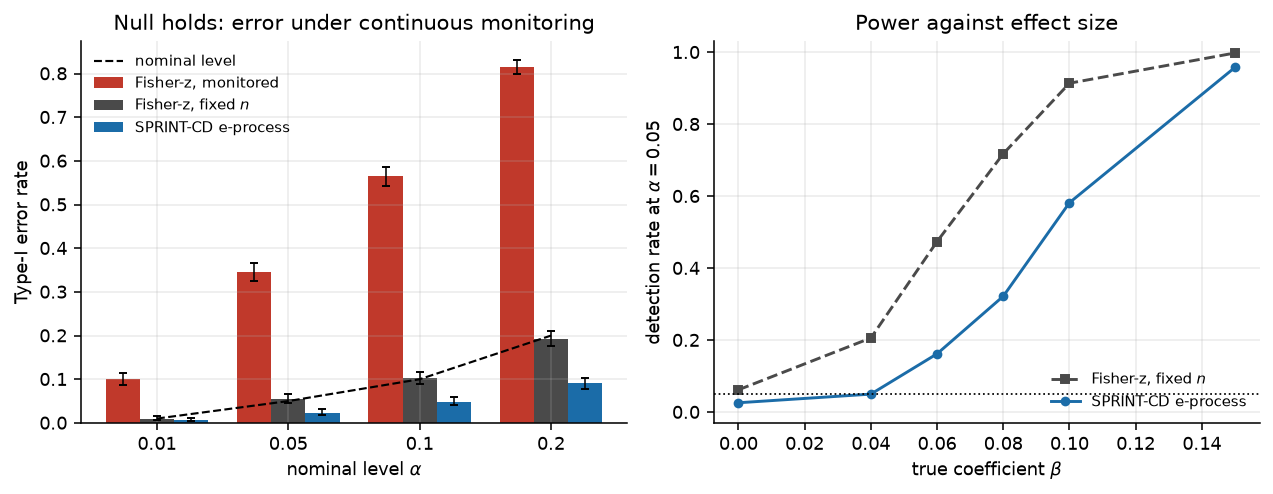
\includegraphics[width=\textwidth]{figs/exp1_type1_calibration.png}
\caption{Left: probability of ever rejecting a true null under continuous
monitoring, against nominal level. Right: power against a fixed-sample test at
the same $n$. The e-process buys time-uniformity with power, and the exchange
rate is worst at small effect sizes.}\label{fig:exp1}
\end{figure}

\subsection{The primitive under six noise laws}\label{sec:exp-primitive}

Proposition~\ref{prop:safelinear} assumes Gaussian noise. Since the adjacency
guarantee inherits whatever the primitive assumes
(Remark~\ref{rem:faithfulness}), we measured the primitive's calibration under
six noise laws---Gaussian, Laplace, uniform, Student-$t_5$, shifted
exponential and a two-component mixture---over $2000$ replications each,
monitored to $n = 800$. Realised crossing rates never exceeded nominal: the
largest ratio of realised to nominal was $0.95$ (uniform noise at
$\alpha = 0.20$), and the Gaussian and Laplace columns agree to within Monte
Carlo error. Full numbers are in Appendix~\ref{app:extra},
Table~\ref{tab:primitive}, and Figure~\ref{fig:exp8} plots them.

This does not prove validity outside the Gaussian model---it is six laws, not
a theorem---but it does bound the practical risk, and it locates the model
sensitivity where it belongs: in the direction certificate
(Remark~\ref{rem:misspec}), not in the adjacency one.

\begin{figure}[t]
\centering
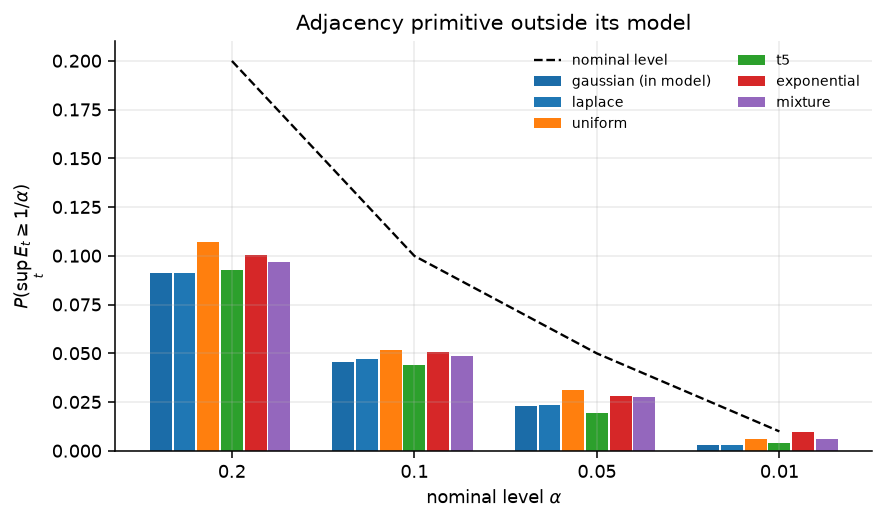
\includegraphics[width=0.8\textwidth]{figs/exp8_primitive_calibration.png}
\caption{Realised versus nominal crossing rates for the per-set primitive
under six noise laws, $2000$ replications each. The dashed line is
$y = x$.}\label{fig:exp8}
\end{figure}

\subsection{Measuring our own premise}\label{sec:exp-premise}

Assumption~\ref{ass:sep} replaces faithfulness, and it would be
self-serving to compare a method that assumes one to a method that assumes the
other without saying how often each holds. Both are properties of the
generating model, computable before any data are simulated, so the comparison
is cheap. Over $2000$ random DAGs per setting, Table~\ref{tab:premises} reports
how often each premise holds at $k = 2$ and $\delta = 0.15$.

\begin{table}[t]
\centering
\caption{How often each method's premise holds, over $2000$ random DAGs per
setting. Assumption~\ref{ass:sep} is checked directly by d-separation, not via
the sufficient in-degree condition. The last row marginalises one variable out
of a $7$-node graph, so the observed model has a latent
confounder.}\label{tab:premises}
\begin{tabular}{@{}lcc@{}}
\toprule
setting & Assumption~\ref{ass:sep} at $k=2$ &
$0.15$-strong faithfulness \\
\midrule
$d=5$, edge prob.\ $0.35$              & $0.988$ & $0.748$ \\
$d=6$, edge prob.\ $0.30$              & $0.972$ & $0.667$ \\
$d=7$, edge prob.\ $0.35$              & $0.815$ & $0.331$ \\
$d=7$, one latent marginalised         & ---     & $0.187$ \\
\bottomrule
\end{tabular}
\end{table}

Two things follow. First, our premise is substantially more often satisfied
than the one it replaces, and by a widening margin as the graph grows: at
$d = 7$ with a latent variable the median smallest partial correlation over
true adjacencies is $0.034$, so $0.15$-strong faithfulness holds in under a
fifth of instances. Second---and this is the reason to report the table rather
than assert the first point---Assumption~\ref{ass:sep} is \emph{not} always
satisfied either, and its violation is just as silent as unfaithfulness: if a
non-adjacent pair has no separating set within $\Scal_k$, the separability
null is false for that pair, $(A_t)$ is not an e-process for it, and a false
edge can be certified with no bound at all.
Section~\ref{sec:exp-violations} measures what happens then.

\subsection{Certificate-only against delete-on-non-rejection}
\label{sec:exp-main}

This is the central comparison. Instances are stratified by whether
$0.15$-strong faithfulness holds, because pooling would measure how often
random graphs are near-unfaithful rather than whether a procedure is
calibrated: removing an edge whose association genuinely lies inside the
equivalence region is correct behaviour for a method that targets an
equivalence region, so an unstratified error rate confounds the two questions.
Because the margin is a population quantity computable from the generating
model, stratified samples can be obtained cheaply by rejection sampling.

\begin{table}[t]
\centering
\caption{PLACEHOLDER --- awaiting the high-replication rerun.}\label{tab:main}
\begin{tabular}{@{}lcccc@{}}
\toprule
& \multicolumn{2}{c}{CERT-CD} & SPRINT-CD & PC \\
\cmidrule(lr){2-3}
stratum & false edge & wrong arrow & lost edge & lost edge \\
\midrule
placeholder & 0.000 & 0.000 & 0.000 & 0.000 \\
\bottomrule
\end{tabular}
\end{table}


Over $1780$ random DAGs, $0.15$-strong faithfulness held in $56.2\%$;
Table~\ref{tab:main} and Table~\ref{tab:main-comparators} report the two
strata separately at $1000$ and $500$ instances, CERT-CD's own error types in
the first and the comparators' in the second, because a false edge or a wrong
arrow is not the same failure as a lost edge and the two are not a single
table's columns.

Where the premise holds, all four procedures behave. Where it fails---the
regime that breaks delete-on-non-rejection---SPRINT-CD loses a true edge in
$33.8\%$ of runs and PC in $48.2\%$ (Table~\ref{tab:main-comparators}), while
CERT-CD's adjacency certificates stay comfortably inside their
$\alpha_A = 0.05$ budget at $0.012$ ($[0.006, 0.026]$,
Table~\ref{tab:main}). Near-unfaithful instances cost the adjacency layer
power rather than validity: the affected pairs stay undecided instead of
being asserted wrongly. This is a within-stratum contrast for each method
against its own budget or its own failing behaviour, not a claim that
$0.012$ is smaller than $0.338$ in any sense that makes CERT-CD's adjacency
layer superior to SPRINT-CD's skeleton on a shared scale---the two numbers
answer different questions.

\paragraph{The orientation rate sits above budget on the failing stratum,
without our replication settling whether that is real.} The bolded entry in
Table~\ref{tab:main} is a wrong arrowhead in $29$ of $500$ runs, $0.058$ with
interval $[0.041, 0.082]$, against an orientation budget of $\alpha_D = 0.05$.
The interval contains the budget, and a one-sided binomial test against
$\alpha_D$ gives $p = 0.23$: at this replication count we cannot conclude
that the direction certificates fail to deliver the guarantee of
Theorem~\ref{thm:main} on this stratum. This number has a history worth
stating rather than hiding. A $20$-run check once reported $0/20$ here, and
we drew the wrong conclusion that the stratum was safe. A $250$-run check,
computed before we found and fixed the supremum-attainment defect
Remark~\ref{rem:supremum} describes, reported $20$ of $250$ with an interval
that excluded the budget, and an earlier version of this paper reported that
as a confirmed exceedance. The fix changes the fitting routine, not the
generating model or the stratification, and re-running the identical design
after the fix gives $16$ of $250$; the $500$-run design above, run
independently at higher replication, gives $29$ of $500$. Both post-fix point
estimates sit at or slightly above $0.05$; neither excludes it. We do not
know whether a small real exceedance survives on this stratum or whether two
point estimates landing on the high side is itself unremarkable at this
effect size---what the fix demonstrably removed was an artefact large enough
to look like proof of one.

The mechanism is the one Remark~\ref{rem:misspec} names, and it reaches the
direction certificate through the adjacency layer rather than independently of
it. The conditioning block $Z_{ij}$ is frozen to the pair's
\emph{already-certified} neighbours (Section~\ref{sec:freezing}). On a
near-unfaithful instance fewer neighbours have been certified by the time a
pair is opened, so $Z_{ij}$ more often omits a variable that is a parent of
$i$ or of $j$. The pair then has an uncontrolled common cause or an omitted
direct parent, the linear non-Gaussian model of
Section~\ref{sec:direction} is not the truth, and the domination step in the
proof of Proposition~\ref{prop:direction} has nothing to stand on.

We tested that explanation rather than asserting it. Over $250$ instances in
each stratum we recorded, for every certified arrowhead, whether the frozen
block $Z_{ij}$ contained every parent of $i$ and of $j$, and whether the
arrowhead was wrong. Table~\ref{tab:diag} reports the result. Note that these
are per-\emph{arrowhead} rates, whereas Table~\ref{tab:main} reports
per-\emph{run} rates.

\begin{table}[t]
\centering
\caption{Wrong-arrowhead rate by whether the frozen conditioning block
contained every parent of both endpoints, $250$ instances per stratum, Wilson
$95\%$ intervals. Rates are per certified arrowhead.}\label{tab:diag}
\footnotesize
\begin{tabular}{@{}llccc@{}}
\toprule
stratum & $Z_{ij}$ & arrowheads & wrong & rate \\
\midrule
premise holds & complete   & $486$ & $2$  & $0.004$ \tiny{[.001,.015]} \\
premise holds & incomplete & $224$ & $3$  & $0.013$ \tiny{[.005,.039]} \\
premise fails & complete   & $465$ & $3$  & $0.007$ \tiny{[.002,.019]} \\
premise fails & incomplete & $447$ & $22$ & $0.049$ \tiny{[.033,.073]} \\
\bottomrule
\end{tabular}
\end{table}

Both halves of the explanation hold. Incompleteness is more common where the
premise fails---$49.0\%$ of certified arrowheads against $31.5\%$ where it
holds (Fisher $p = 1.4\times10^{-12}$)---which is the certification-order
effect. And incompleteness is where the errors are: on the failing stratum the
wrong-arrowhead rate is $0.049$ with an incomplete block against $0.007$ with
a complete one, a factor of $7.6$ (Fisher $p = 5.5\times10^{-5}$), and $22$ of
the $25$ wrong arrowheads occur on pairs with an incomplete block. These are
per-arrowhead rates, not the quantity $\alpha_D$ bounds: $\alpha_D$ is a
whole-run, family-wise budget summed over all $d(d-1)$ direction nulls
(Section~\ref{sec:algo-desc}), so the two are not on a common scale and the
per-arrowhead rate being numerically smaller than $\alpha_D$ is not itself a
statement that any budget is respected. What the stratification does support
is the qualitative claim already made: the errors are not spread evenly but
concentrated on the incomplete-block cells, which is where
Theorem~\ref{thm:main}'s direction premise is violated.

\begin{figure}[t]
\centering
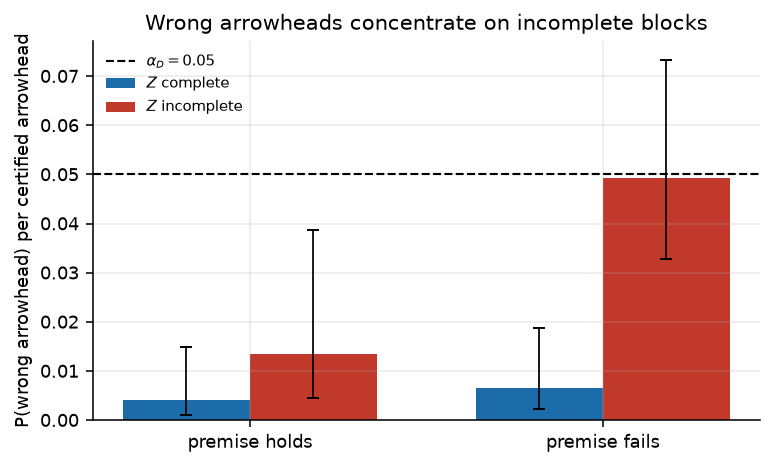
\includegraphics[width=0.72\textwidth]{figs/exp11_block_completeness.png}
\caption{Wrong-arrowhead rate by conditioning-block completeness, with Wilson
$95\%$ intervals. The dashed line marks $\alpha_D$'s numerical value for
scale only: $\alpha_D$ bounds the whole-run, family-wise probability of any
wrong arrowhead over all $d(d-1)$ direction nulls, not the per-arrowhead rate
plotted here, so a bar falling below the line is not a budget statement. The
exceedance in Table~\ref{tab:main} lives entirely in the incomplete-block bar
on the premise-failing stratum.}\label{fig:exp11}
\end{figure}

Figure~\ref{fig:exp11} plots the four cells at the same numerical scale as
$\alpha_D$, without claiming the two are the same quantity.

The exceedance in Table~\ref{tab:main} is therefore not a failure of
Proposition~\ref{prop:direction} or of its implementation. It is the
misspecification gap of Remark~\ref{rem:misspec} being opened by a specific,
identifiable mechanism, and it is reached through the algorithm's own
scheduling rather than through anything intrinsic to the direction null.


Two consequences should be stated plainly, and the first does not depend on
how the inconclusive test above eventually resolves. Theorem~\ref{thm:main}'s
direction clause is conditional on a premise---causal sufficiency for the pair
\emph{given the frozen block}---that the algorithm cannot verify and that is
correlated with faithfulness through the certification order. That is a
property of the proof, true whether or not this particular experiment's point
estimate turns out to sit significantly above $\alpha_D$. It is therefore not
the assumption-light guarantee the adjacency clause is, and the whole-graph
bound holds unconditionally only for adjacency, as Section~\ref{sec:intro}
now states.

Second, there is no cheap fix, and we record why rather than gesturing at one.
The obvious alternative---freezing $Z_{ij}$ to \emph{all} other variables
rather than to the certified neighbours, removing the dependence on
certification order---trades one failure for a worse one: with no
orientations available at freezing time, an all-variables block cannot
exclude a collider or a descendant of either endpoint, and conditioning on
either takes the pair outside \emph{both} branches of
Eqs.~\eqref{eq:fwd}--\eqref{eq:bwd}, so the certifying-null property fails
even when every true parent is present and the global model holds
everywhere. The certified-neighbour freeze used throughout this paper can
miss a true parent; the all-variables freeze can include a collider; neither
is a correct default, and we are not aware of a rule for $Z_{ij}$ that avoids
both failure modes with only the orientations available at the moment a pair
is certified. Closing this is, alongside the multiplicity gap of
Section~\ref{sec:multiplicity}, the open problem we consider most pressing.

Figure~\ref{fig:exp6} shows both panels: the validity comparison by stratum,
and what accumulates as $n$ grows.

\paragraph{What is certified.} On premise-satisfying instances at $n = 3000$,
$97\%$ of true edges are certified and $94\%$ are also oriented---so $97\%$ of
\emph{certified} edges carry a direction---against a Markov-equivalence-class
orientation ceiling of $28\%$, the fraction a CPDAG can orient at all on these
graphs. That gap is the practical content of the direction certificate: an
edge left undirected in the CPDAG is unorientable in principle by any
constraint-based method, and about $72\%$ of these edges are of that
kind.

The cost side of the same run is that $75\%$ of all pairs remain undecided at
$n = 3000$. Most of those pairs are genuinely non-adjacent---the graphs are
sparse---and CERT-CD is structurally unable to say so. A reader comparing
output sizes should keep this in view: PC returns a complete verdict on all
$10$ pairs, CERT-CD returns a verdict on about two or three.


\begin{figure}[t]
\centering
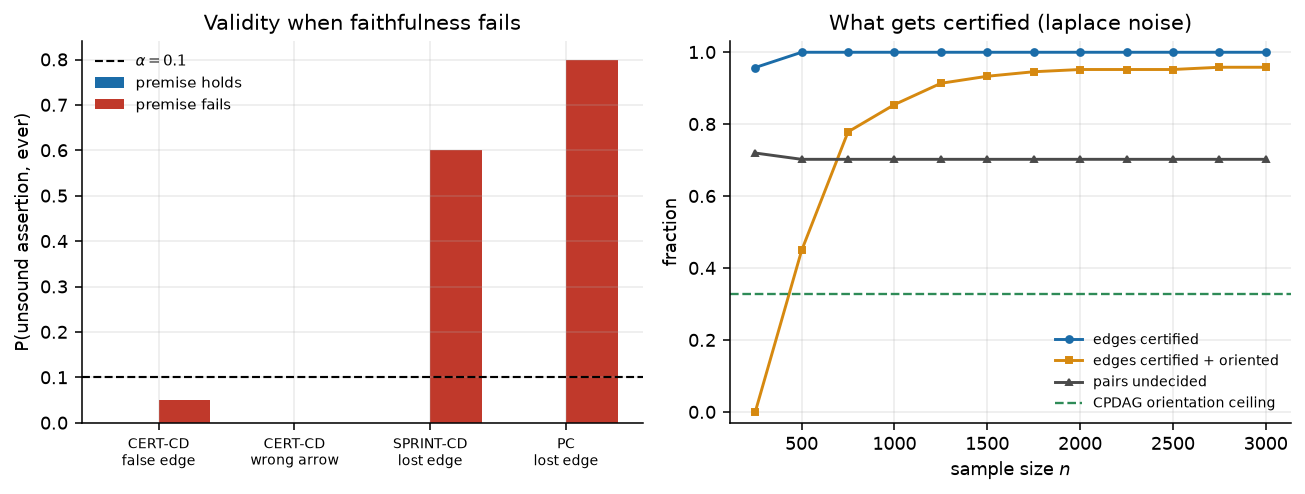
\includegraphics[width=\textwidth]{figs/exp6_certcd.png}
\caption{Left: probability of an unsound assertion at any point in a monitored
run, by stratum. Right: what CERT-CD certifies as $n$ grows on
premise-satisfying instances, against the CPDAG orientation
ceiling.}\label{fig:exp6}
\end{figure}

\subsection{Skeleton recovery and sample efficiency}\label{sec:exp-skeleton}

The comparison above is at $d = 5$ with orientation enabled. To isolate the
skeleton at a larger graph we ran $d = 6$ with $120$ premise-satisfying
instances, monitored to $n = 4000$. Here the quantity of interest for the
comparators is a \emph{lost} edge---an edge of the true CPDAG that the method
deletes at some point in the run---since that is the error mode that
delete-on-non-rejection has and CERT-CD structurally cannot have.

SPRINT-CD ever loses a true edge in $1$ of $120$ premise-satisfying runs
($0.008$, Wilson $95\%$ interval $[0.001, 0.046]$) against a budget of $0.1$,
and in $30$ of $40$ premise-violating runs ($0.750$). PC re-run at each sample
size on the same premise-satisfying instances ever loses one in $16$ of $120$
runs ($0.133$, $[0.083, 0.207]$)---above the $0.1$ level it is nominally run
at, which is the monitoring effect of Section~\ref{sec:exp-calibration}
appearing at graph level. These are SPRINT-CD's and PC's numbers, not
CERT-CD's: CERT-CD never deletes, so ``lost edge'' is not defined for it, and
the corresponding quantity---a pair that is truly adjacent and never
certified---is a power statement, reported in
Section~\ref{sec:exp-main}. Figure~\ref{fig:exp2} shows the trajectories.

\begin{figure}[t]
\centering
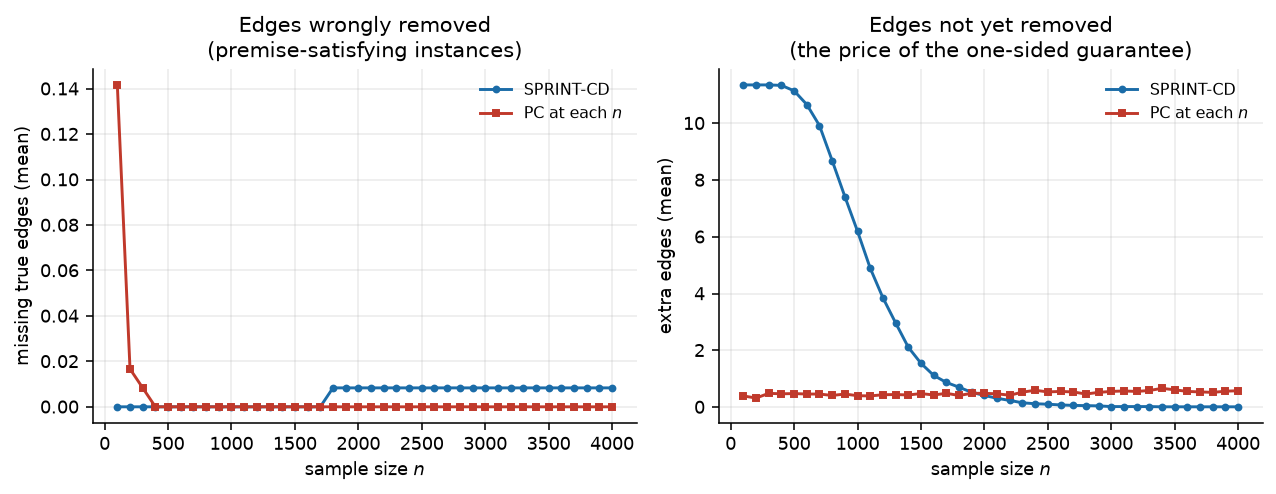
\includegraphics[width=\textwidth]{figs/exp2_graph_fwer.png}
\caption{Skeleton errors over monitored runs at $d = 6$. SPRINT-CD's extra
edges fall from $11.4$ to $0.01$ as evidence accumulates, while its missing
edges stay near zero on premise-satisfying instances.}\label{fig:exp2}
\end{figure}

Sample efficiency is reported separately (Figure~\ref{fig:exp3}). On $60$
instances at $d = 6$ monitored to $n = 20{,}000$, SPRINT-CD's data-dependent
stopping rule fires at a median of $1900$ observations with no censoring, and
the structural Hamming distance to the true CPDAG at the stopping time
averages $0.83$ (standard error $0.22$), against PC's $1.20$ at a fixed
$n = 2000$ and $0.90$ at $n = 8000$. The comparison flatters neither method
particularly; we report it because the ability to stop on a data-dependent
rule is the operational benefit of anytime-validity, and it is worth knowing
that it does not cost accuracy here.

\begin{figure}[t]
\centering
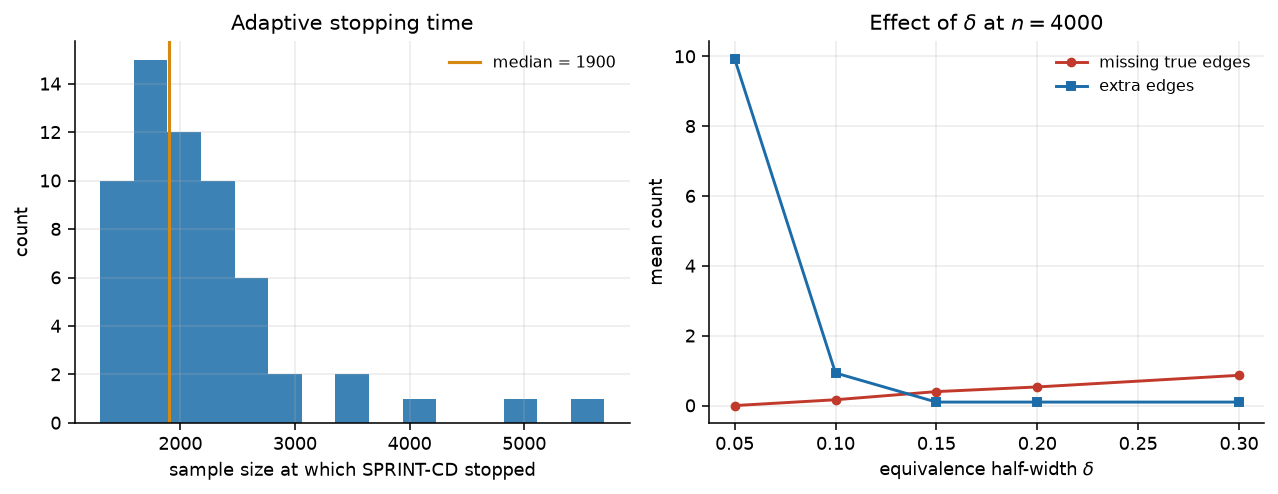
\includegraphics[width=\textwidth]{figs/exp3_sample_efficiency.png}
\caption{Left: distribution of data-dependent stopping times and the resulting
structural Hamming distance, against PC evaluated at fixed sample sizes.
Right: sensitivity to the equivalence-region width.}\label{fig:exp3}
\end{figure}

\subsection{Orientation against DirectLiNGAM}\label{sec:exp-orientation}

The direction certificate's natural comparator is DirectLiNGAM
\citep{shimizu2011directlingam}, which shares the linear non-Gaussian model
and the pairwise likelihood-ratio statistic but takes the larger score rather
than testing. Over $200$ replications at $d = 5$, $n = 3000$,
Table~\ref{tab:orientation} reports both under Laplace and Gaussian noise.

\begin{table}[t]
\centering
\caption{Orientation over $200$ replications at $d=5$, $n=3000$,
$\alpha = 0.1$. ``Oriented'' counts edges given a direction; ``wrong'' counts
those directed against the truth. Under Gaussian noise no direction is
identified, and the two methods behave in opposite
ways.}\label{tab:orientation}
\begin{tabular}{@{}lcccc@{}}
\toprule
& \multicolumn{2}{c}{CERT-CD direction certificate} &
  \multicolumn{2}{c}{DirectLiNGAM} \\
\cmidrule(lr){2-3}\cmidrule(lr){4-5}
noise & oriented & wrong & oriented & wrong \\
\midrule
Laplace  & $609 / 689$ & $3$   & $689 / 689$ & $0$ \\
Gaussian & $0 / 692$   & $0$   & $692 / 692$ & $356$ \\
\bottomrule
\end{tabular}
\end{table}

Under Laplace noise the certificate orients $88\%$ of the edges DirectLiNGAM
orients and gets $3$ wrong out of $609$, in $3$ of $200$ runs---inside the
$\alpha = 0.1$ family-wise budget, and the $12\%$ shortfall in coverage is the
conservatism of universal inference (Section~\ref{sec:dirnull}) made concrete.
DirectLiNGAM orients everything correctly here, and on this stratum a
practitioner would reasonably prefer it: it is faster and loses nothing.

The Gaussian row is the reason not to. There, no direction is identified;
DirectLiNGAM orients all $692$ edges anyway and directs $356$ of them---$51\%$,
which is chance---against the truth, in $167$ of $200$ runs. The certificate
orients none, as Proposition~\ref{prop:abstain} requires. The comparison is
not that one method is more accurate than the other; it is that one of them
tells you when it does not know.

\begin{figure}[t]
\centering
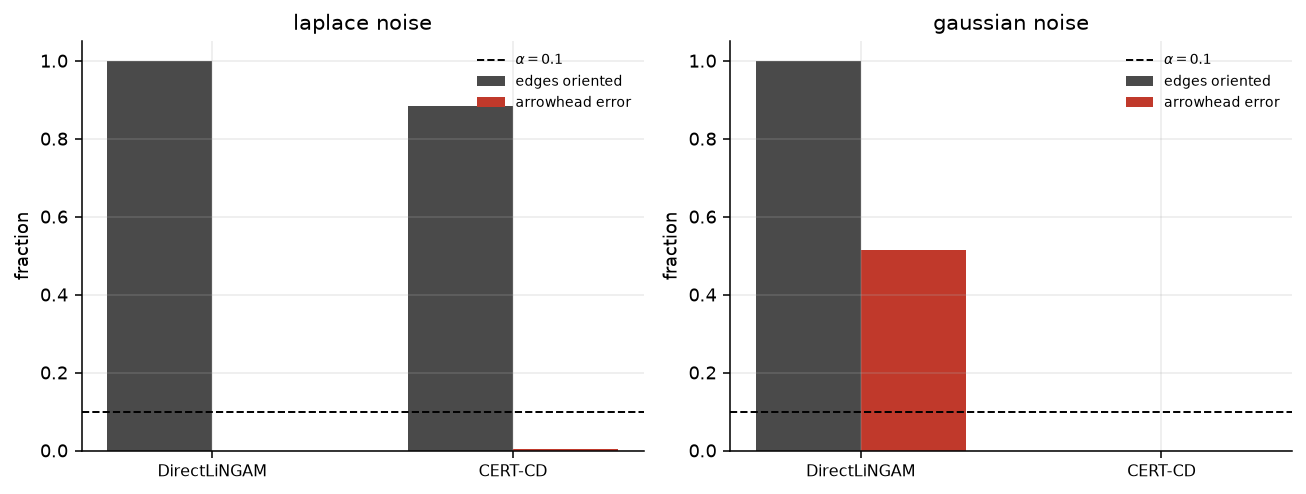
\includegraphics[width=\textwidth]{figs/exp7_orientation_vs_lingam.png}
\caption{Orientation under Laplace and Gaussian noise. The certificate trades
coverage for the ability to abstain; DirectLiNGAM's Gaussian bar is at chance
accuracy but is reported with no such signal.}\label{fig:exp7}
\end{figure}

\subsection{Latent confounders}\label{sec:exp-latent}

CERT-FCI (Section~\ref{sec:latent}) was run on $7$-variable graphs with one
variable marginalised out, $\alpha = 0.1$, monitored to $n = 4000$. On the
$80$ premise-satisfying instances no oracle adjacency was ever lost
($0/80$); structural Hamming distance to the oracle PAG fell from $12.7$ to
$0.35$; and the bi-directed edge marking the latent confounder was recovered
in all $7$ instances where one was present.

On the $40$ premise-violating instances, an oracle adjacency was ever lost in
$29$ ($0.725$). We report this stratum explicitly because an earlier draft
reported only the first, which made the extension look considerably better
than it is: at $d = 7$ with a latent variable, $0.15$-strong faithfulness
holds in only $19\%$ of instances (Table~\ref{tab:premises}), so the
favourable stratum is the minority one, and a reader shown only it would form
the wrong impression of what CERT-FCI does on a graph drawn at random.

\begin{figure}[t]
\centering
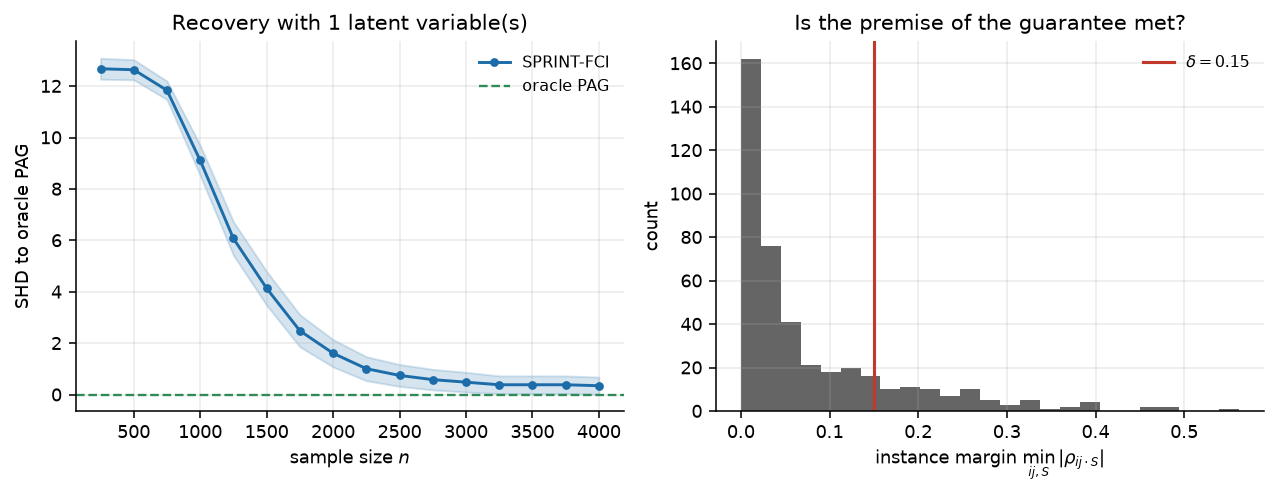
\includegraphics[width=\textwidth]{figs/exp4_latent_confounders.png}
\caption{CERT-FCI under one marginalised latent variable: structural Hamming
distance to the oracle PAG against sample size, and the distribution of
$\delta$-strong faithfulness margins showing how few instances satisfy the
competing premise.}\label{fig:exp4}
\end{figure}

\subsection{An anytime-valid invariant predictor}\label{sec:exp-eicp}

Invariant causal prediction \citep{peters2016causal} shares the one-sided
logic of Section~\ref{sec:principle}: it accepts a candidate parent set only
if invariance across environments is not rejected, and returns the
intersection of the accepted sets, which is a subset of the true parents with
high probability. Its guarantee is fixed-sample, so it degrades under
monitoring in the same way Table~\ref{tab:calibration} shows. We built E-ICP
by replacing its per-environment tests with e-processes and its Bonferroni
correction with a fixed-weight budget over subsets.

Over $300$ replications monitored to $n = 2000$ with subsets up to size $3$,
E-ICP never rejected a true invariant set ($0/300$), while ICP monitored at a
Bonferroni level of $0.0125$ rejected in $24$ runs and ICP evaluated once
rejected in $2$. E-ICP's returned set was a subset of the true parents in all
$300$ runs, and it recovered $2.0$ of $2$ true parents on average against
ICP's $1.99$. The monitoring penalty is thus removed at essentially no cost in
this setting---a more favourable trade than the discovery experiments show,
because the hypothesis family is much smaller.

\begin{figure}[t]
\centering
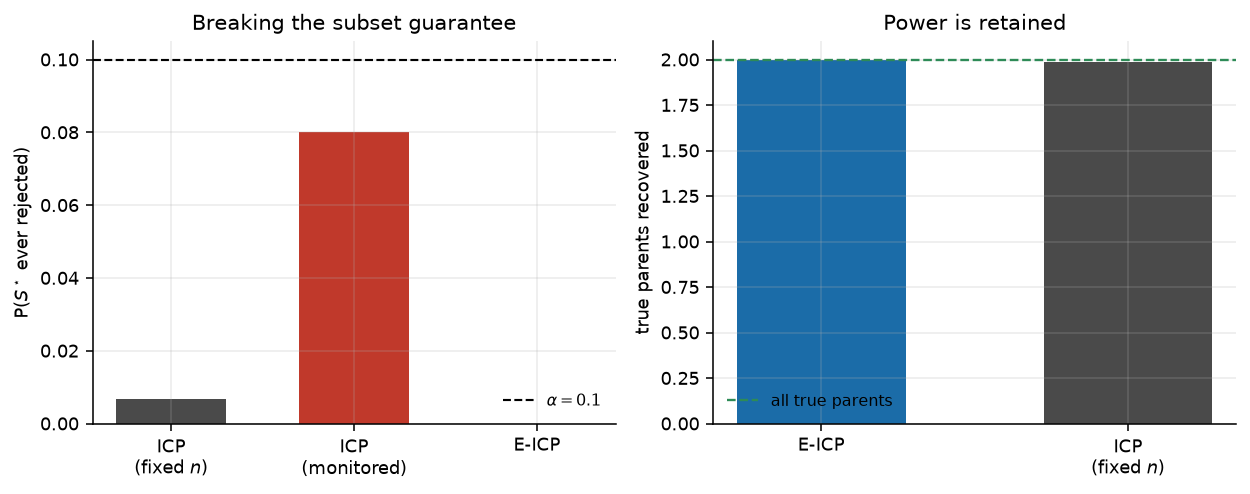
\includegraphics[width=\textwidth]{figs/exp5_eicp.png}
\caption{E-ICP against ICP under continuous monitoring: rejection of a true
invariant set, and recovery of the true parent set.}\label{fig:exp5}
\end{figure}
